\chapter{Experimental Evaluation}\label{c:evaluations}



We measured the runtime performance of our privacy\hyp preserving algorithms using the Sharemind secure computing platform.
We instantiated all private aggregators and decision tree classifiers using the SecreC programming language \cite{jagomagis2010secrec} that Sharemind provides.
In Sharemind, the number of the computing parties are restricted by the SMPC protocol that is been used.
Our experiments use the \textit{pd\_shared3p} security protocol, which utilizes three nodes in the private domain.


Below, we present the experimental evaluation timings of the developed privacy\hyp preserving histograms and decision trees.
Our goal is to provide a concise and holistic view of our experiments\footnote{All time measurements presented in this section correspond to the sole privacy computation. The importing timings were roughly 1 second, even for the largest dataset, thus we did not take it into account in the graphs.}, by carefully select the most descriptive diagrams.


\textbf{Experimental Setup:}
All experiments were performed on three 64-bit virtual machines (VM), each running Ubuntu 18.04.
The three VMs share an Intel Xeon E5-2670 (v2) at 2.50 GHz.
Each VM utilizes 6 cores and 8 GB of memory.


\section{Histograms}\label{s:results-histograms}

The first experimental timing results are about the privacy\hyp preserving histogram computations.
In figure \ref{chart:numerical-histogram} we show the scaling in execution time of histograms on numerical data.
In figure \ref{chart:categorical-histogram} we exhibit the respective measurements for histograms on categorical data.
\textit{Note:} both $x$ and $y$ axes are log\hyp scaled.


\begin{figure}[H]
\centering
\centerline{
\begin{minipage}{.5\linewidth}
  \centering
  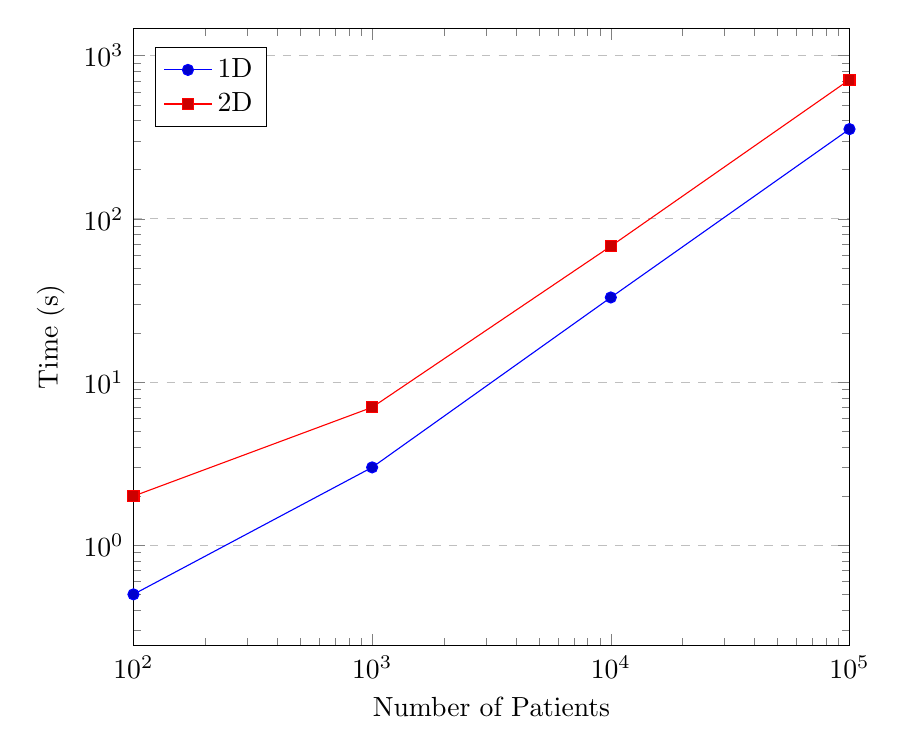
\begin{tikzpicture}
  \begin{axis}[
    legend pos=north west,
    scale only axis,
    enlarge x limits=-1,
    width=\textwidth*0.75,
    ymajorgrids=true,
    xmode=log,
    ymode=log,
    % log ticks with fixed point,
    xlabel={Number of Patients},
    ylabel={Time (s)},
    ymin=0,
    grid style=dashed
  ]
  \addplot
    coordinates {(100, 0.5)(1000, 3)(10000, 33)(100000, 355)};
    \addlegendentry{1D}
  \addplot
    coordinates {(100, 2)(1000, 7)(10000, 68)(100000, 713)};
    \addlegendentry{2D}
  \end{axis}
  \end{tikzpicture}
  \caption{Numerical histograms timings}\label{chart:numerical-histogram}
\end{minipage}%
\begin{minipage}{.5\linewidth}
  \centering
  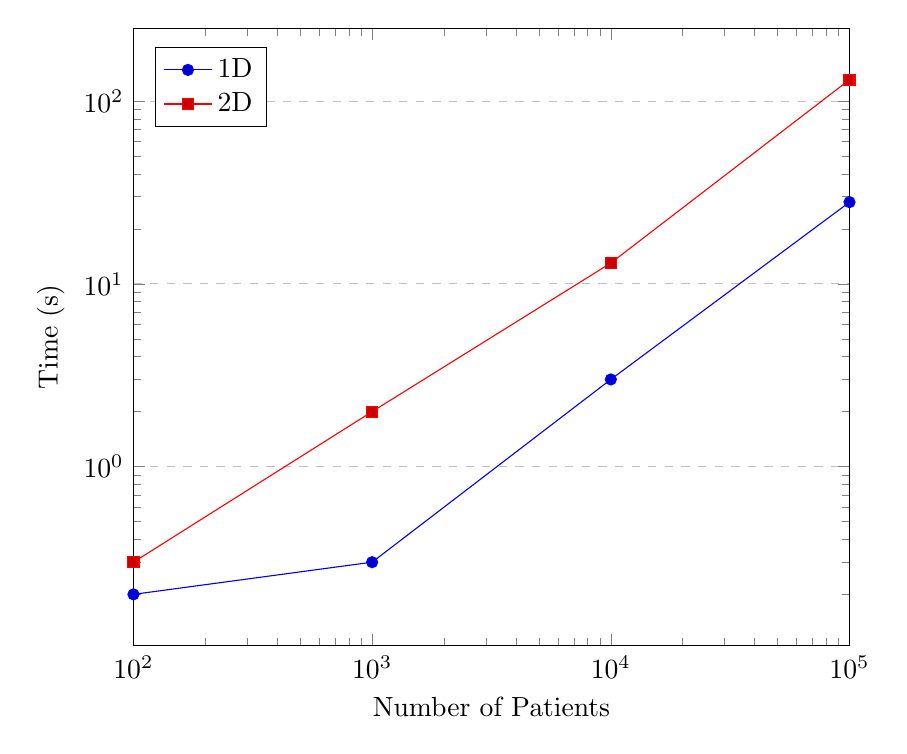
\begin{tikzpicture}
  \begin{axis}[
    legend pos=north west,
    scale only axis,
    enlarge x limits=-1,
    width=\textwidth*0.75,
    ymajorgrids=true,
    xmode=log,
    ymode=log,
    % log ticks with fixed point,
    xlabel={Number of Patients},
    ylabel={Time (s)},
    ymin=0,
    grid style=dashed
  ]
  \addplot
    coordinates {(100, 0.2)(1000, 0.3)(10000, 3)(100000, 28)};
    \addlegendentry{1D}
  \addplot
    coordinates {(100, 0.3)(1000, 2)(10000, 13)(100000, 131)};
    \addlegendentry{2D}
  \end{axis}
  \end{tikzpicture}
  \caption{Categorical histograms timings}\label{chart:categorical-histogram}
\end{minipage}
}
\end{figure}

One can observe that the histograms on categorical data perform better than their numerical data equivalents, especially when applied over bigger datasets.
This is due to the extra computation that needs to be done in the case of numerical data, in order to determine the corresponding histogram cell for each data tuple.
Moreover, the privacy\hyp preserving histograms scale linearly with the dataset size, regardless the type of it.

The chart below (figure \ref{chart:numerical-histogram-filters}) depicts the timings of histograms on numerical data (such as figure \ref{chart:numerical-histogram}), but also with the application of some filters / constraints.
We can clearly see that as the dataset size grows, the number of filters does not make much of a difference in the total algorithm's execution time.

%%%%%%%%%%%%%%%%%%%%%%%%%%%%%%%%%%%%%%%%%%%%%%%%%%%%%%%%%%%%%%%%%%%%%%%%%%%%%%%%%%%

\begin{figure}[H]
\centering
\centerline{
\begin{minipage}{.8\linewidth}
  \centering
  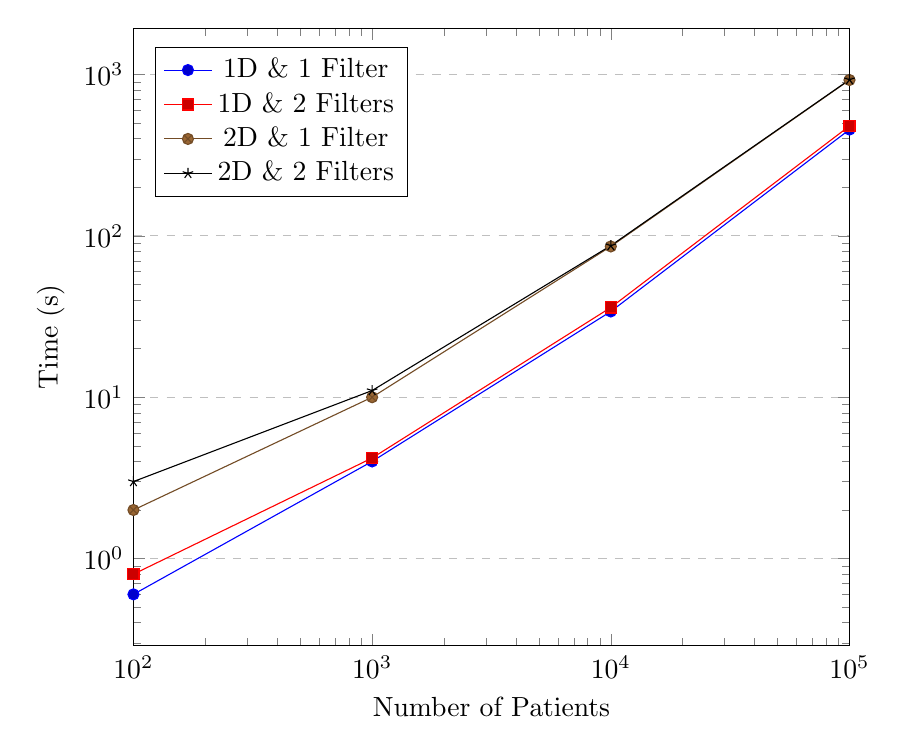
\begin{tikzpicture}
  \begin{axis}[
    legend pos=north west,
    scale only axis,
    enlarge x limits=-1,
    width=\textwidth*0.75,
    ymajorgrids=true,
    xmode=log,
    ymode=log,
    % log ticks with fixed point,
    xlabel={Number of Patients},
    ylabel={Time (s)},
    ymin=0,
    grid style=dashed
  ]
  \addplot
    coordinates {(100, 0.6)(1000, 4)(10000, 34)(100000, 456)};
    \addlegendentry{1D \& 1 Filter}
  \addplot
    coordinates {(100, 0.8)(1000, 4.2)(10000, 36)(100000, 480)};
    \addlegendentry{1D \& 2 Filters}
  \addplot
    coordinates {(100, 2)(1000, 10)(10000, 86)(100000, 925)};
    \addlegendentry{2D \& 1 Filter}
  \addplot
    coordinates {(100, 3)(1000, 11)(10000, 87)(100000, 929)};
    \addlegendentry{2D \& 2 Filters}
  \end{axis}
  \end{tikzpicture}
  \caption{Numerical histograms with filters timings}\label{chart:numerical-histogram-filters}
\end{minipage}%
}
\end{figure}


%%%%%%%%%%%%%%%%%%%%%%%%%%%%%%%%%%%%%%%%%%%%%%%%%%%%%%%%%%%%%%%%%%%%%%%%%%%%%%%%%%%
%%%%%%%%%%%%%%%%%%%%%%%%%%%%%%%%%%%%%%%%%%%%%%%%%%%%%%%%%%%%%%%%%%%%%%%%%%%%%%%%%%%
%%%%%%%%%%%%%%%%%%%%%%%%%%%%%%%%%%%%%%%%%%%%%%%%%%%%%%%%%%%%%%%%%%%%%%%%%%%%%%%%%%%

\newpage
\section{Decision Trees}\label{s:results-dtrees}
Consecutively, we measured the privacy\hyp preserving classification algorithms.
For the sake of simplicity\footnote{Privacy\hyp preserving C4.5 and ID3 algorithms scale similarly, however the overall timings of C4.5 are more time consuming.}, we present the timings of the ID3 algorithm.\footnote{
Textbook C4.5 algorithm's time complexity \cite{su2006fast} (\bigo{m \cdot n^2}, where $m$ is the size of the training data and $n$ is the number of attributes) renders it impracticable to scale when it is translated to the privacy\hyp preserving domain.
For many classification attributes and a large number of patients, C4.5 has an unbearable runtime overhead.
}
Figure \ref{chart:id3-patients} portrays how the ID3 algorithm scales as the dataset size grows, for a constant number (3) of classification attributes (``Heart rate'', ``Height (cm)'' and ``Patient Age'').
\textit{Note:} both $x$ and $y$ axes are log\hyp scaled.


\begin{figure}[H]
\centering
\centerline{
\begin{minipage}{.5\linewidth}
  \centering
  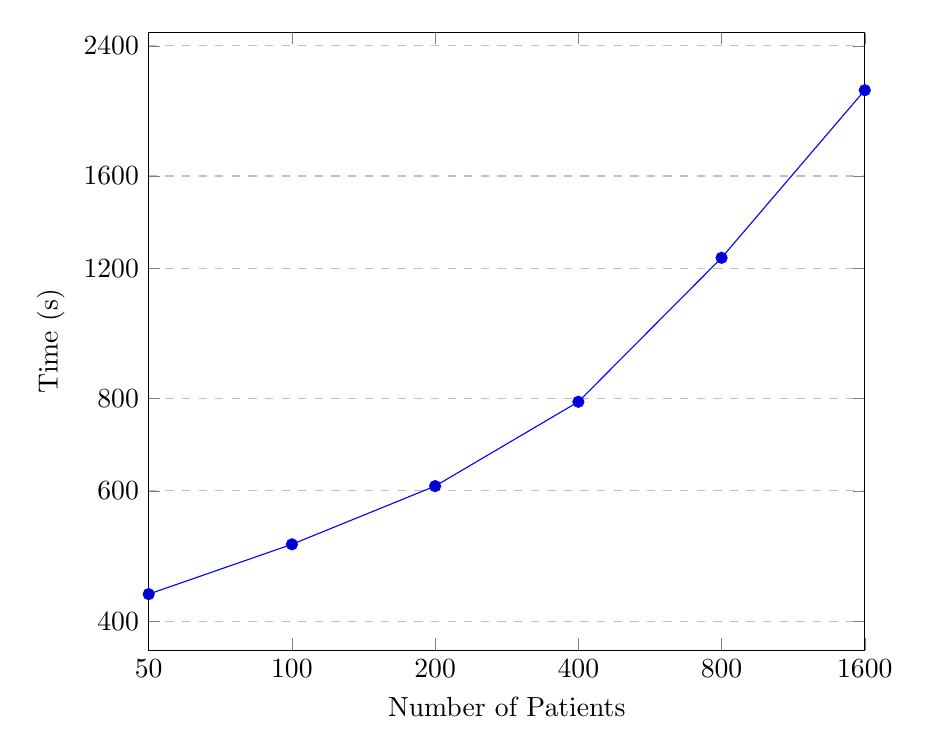
\begin{tikzpicture}
  \begin{axis}[
    legend pos=north west,
    scale only axis,
    enlarge x limits=-1,
    width=\textwidth*0.75,
    ymajorgrids=true,
    xmode=log,
    ymode=log,
    log ticks with fixed point,
    xlabel={Number of Patients},
    ylabel={Time (s)},
    xtick = {50, 100, 200, 400, 800, 1600},
    ytick = {400, 600, 800, 1200, 1600, 2400, 3200},
    ymax=2500,
    grid style=dashed,
    y tick label style={/pgf/number format/.cd,%
          set thousands separator={}},
      x tick label style={/pgf/number format/.cd,%
          set thousands separator={}}%
  ]
  \addplot
    coordinates {(50, 435)(100, 508)(200, 609)(400, 792)(800, 1240)(1600, 2090)};
  \end{axis}
  \end{tikzpicture}
  \caption{ID3 decision tree classifier timings with variable patients for 3 attributes}\label{chart:id3-patients}
\end{minipage}%
\begin{minipage}{.5\linewidth}
  \centering
  \begin{tikzpicture}
  \begin{axis}[
    legend pos=north west,
    scale only axis,
    enlarge x limits=-1,
    width=\textwidth*0.75,
    ymode=log,
    ymajorgrids=true,
    % log ticks with fixed point,
    xlabel={Number of Attributes},
    xtick = {1, 2, 3, 4, 5},
    ylabel={Time (s)},
    ymin=0,
    grid style=dashed
  ]
  \addplot
    coordinates {(1, 107)(2, 509)(3, 1547)(4, 3428)(5, 6835)};
  \end{axis}
  \end{tikzpicture}
  \caption{ID3 decision tree classifier timings with variable number of attributes}\label{chart:id3-attributes}
\end{minipage}
}
\end{figure}



We observe that the execution time of the algorithm is sub\hyp linear regarding the dataset size.


Finally, an overview of the runtime performance of the ID3 algorithm for a constant number of patients and variable number of classification attributes is presented in figure \ref{chart:id3-attributes}.
\textit{Note:} $y$ axis is log\hyp scaled.
As we observe from our experiments, the number of attributes used for classification is a dominating factor in the algorithm's performance.

The execution times for the privacy\hyp preserving creation of the decision trees is orders of magnitude greater than those of equivalent algorithms working on unencrypted data.
However, this is the training part of the classification algorithm which is performed offline.
For this reason, it does not affect the user experience, since training can happen non\hyp interactively at predefined periods of time (\textit{e.g.} every night or once a week).



